\section{Global Network anakysis}
\begin{figure}[h!]
    \centering
    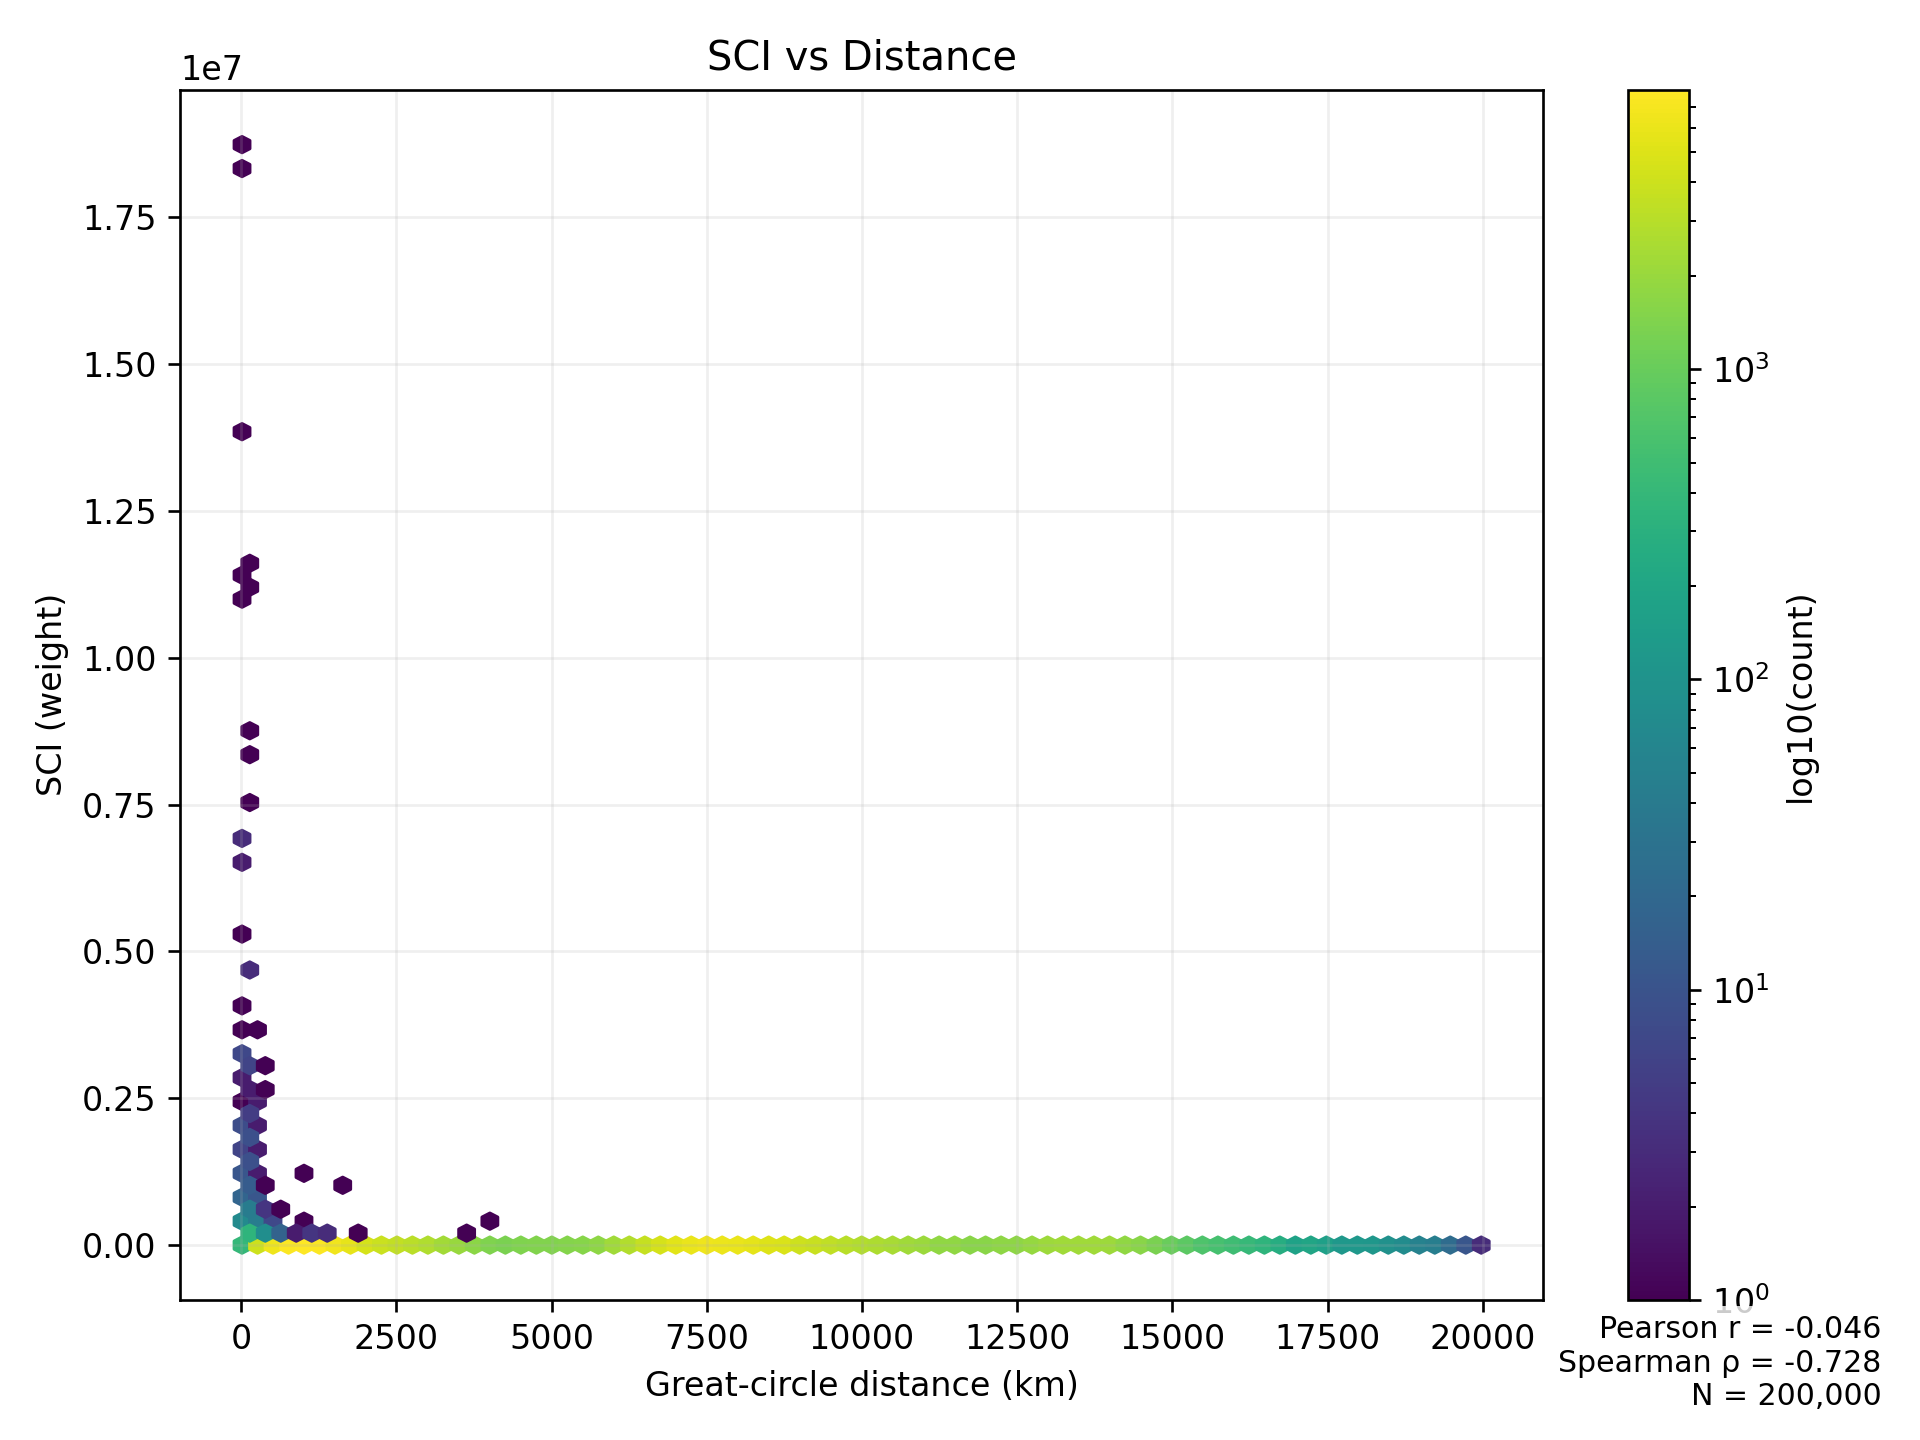
\includegraphics[width=0.65\linewidth]{images/TASK3/global_distance_vs_sci.png}
    \caption{Relationship between SCI weights and great-circle distance. The color scale indicates the log$_{10}$ of the number of pairs.}
    \label{fig:distance}
\end{figure}

\textbf{SCI vs.\ Distance.}  
Figure~\ref{fig:distance} illustrates how social connectedness decreases with geographic distance.
This considers not the network of each country but a random sampling (to have affordable computations, even though could generate a bias and invalidate the results) of the global network.
Most pairs of regions lie in the short-range regime (below $\sim$2000 km), where SCI values are highest and connections most frequent.  
Beyond this range, SCI values drop sharply, confirming a strong distance–decay effect: geographically closer regions are far more likely to be socially connected.  

Despite this general trend, a small number of long-distance pairs retain relatively high SCI values.  
These outliers often reflect historical ties, migration flows, or cultural and linguistic affinities that sustain connections despite large geographic separation.  
The color scale highlights that the majority of pairs correspond to weak ties at short distances, while strong long-distance links are rare but significant.
